\documentclass[11pt]{article}
\usepackage{lmodern}
\usepackage{amssymb,amsmath}
\usepackage{ifxetex,ifluatex}
\usepackage{fixltx2e} % provides \textsubscript
\ifnum 0\ifxetex 1\fi\ifluatex 1\fi=0 % if pdftex
  \usepackage[T1]{fontenc}
  \usepackage[utf8]{inputenc}
\else % if luatex or xelatex
  \ifxetex
    \usepackage{mathspec}
    \usepackage{xltxtra,xunicode}
  \else
    \usepackage{fontspec}
  \fi
  \defaultfontfeatures{Mapping=tex-text,Scale=MatchLowercase}
  \newcommand{\euro}{€}
\fi
% use upquote if available, for straight quotes in verbatim environments
\IfFileExists{upquote.sty}{\usepackage{upquote}}{}
% use microtype if available
\IfFileExists{microtype.sty}{%
\usepackage{microtype}
\UseMicrotypeSet[protrusion]{basicmath} % disable protrusion for tt fonts
}{}
\ifxetex
  \usepackage[setpagesize=false, % page size defined by xetex
              unicode=false, % unicode breaks when used with xetex
              xetex]{hyperref}
\else
  \usepackage[unicode=true]{hyperref}
\fi
\usepackage[usenames,dvipsnames]{color}
\hypersetup{breaklinks=true,
            bookmarks=true,
            pdfauthor={},
            pdftitle={},
            colorlinks=true,
            citecolor=blue,
            urlcolor=blue,
            linkcolor=magenta,
            pdfborder={0 0 0}}
\urlstyle{same}  % don't use monospace font for urls
\usepackage{longtable,booktabs}
\usepackage{graphicx,grffile}
\makeatletter
\def\maxwidth{\ifdim\Gin@nat@width>\linewidth\linewidth\else\Gin@nat@width\fi}
\def\maxheight{\ifdim\Gin@nat@height>\textheight\textheight\else\Gin@nat@height\fi}
\makeatother
% Scale images if necessary, so that they will not overflow the page
% margins by default, and it is still possible to overwrite the defaults
% using explicit options in \includegraphics[width, height, ...]{}
\setkeys{Gin}{width=\maxwidth,height=\maxheight,keepaspectratio}
\setlength{\parindent}{0pt}
\setlength{\parskip}{6pt plus 2pt minus 1pt}
\setlength{\emergencystretch}{3em}  % prevent overfull lines
\providecommand{\tightlist}{%
  \setlength{\itemsep}{0pt}\setlength{\parskip}{0pt}}
\setcounter{secnumdepth}{0}

\date{}

% Redefines (sub)paragraphs to behave more like sections
\ifx\paragraph\undefined\else
\let\oldparagraph\paragraph
\renewcommand{\paragraph}[1]{\oldparagraph{#1}\mbox{}}
\fi
\ifx\subparagraph\undefined\else
\let\oldsubparagraph\subparagraph
\renewcommand{\subparagraph}[1]{\oldsubparagraph{#1}\mbox{}}
\fi

\setlength{\oddsidemargin}{-0.1in}
\setlength{\topmargin}{-0.52truein} 
\setlength{\textheight}{9.15in} 
\setlength{\textwidth}{6.7in}

\usepackage[T1]{fontenc}
\usepackage{fourier}
\usepackage[sc]{mathpazo}
\linespread{1.05}         % Palatino needs more leading (space between lines)
\newcommand\Alfven{Alfv\'en }
\newcommand{\V}[1]{\mathbf{#1}} 


\usepackage{wrapfig}
\usepackage[square,numbers,sort&compress]{natbib}
\renewcommand{\cite}{\citep}
%\usepackage[psamsfonts]{amssymb}
%\usepackage{palatino}
%\usepackage{mathpazo}
\usepackage{plasmadefs}

\hyphenation{wave-packet wave-packets}

\title{}

\begin{document}

\section{Introduction and Motivation}

This renewal proposal requests funds to continue operation of the Basic
Plasma Science Facility (BaPSF) at the University of California, Los
Angeles (UCLA), and to support the vigorous research program of the
BaPSF scientific staff, as well as to continue the improvements in
scientific instrumentation required to maintain worldwide leadership in
fundamental plasma research.  BaPSF provides national and international scientists access to unique
research devices and diagnostic tools that permit the exploration of a
wide range of fundamental plasma problems that impact topics at the
frontiers of fusion, space science and plasma technology. The broad
parameter ranges accessible in the plasma devices operated at BaPSF
allow studies that span microscopic phenomena on the fast electron time
scales (e.g., electron plasma waves, cyclotron radiation) to the slow
time scales characteristic of plasma transport driven by drift-wave
turbulence and long wavelength magnetic fluctuations. This extensive
basic plasma research capability in a single laboratory setting is not
available anywhere else, but examples of analogous user facilities exist
in other scientific disciplines. Qualified researchers and research
teams from universities, national laboratories and industry can perform
experiments at BaPSF, free of charge, upon approval of their proposals
by a Scientific Council composed of senior scientists broadly
representative of the plasma community.

Over the past 5 years, the scientific activities at BaPSF involve
individuals affiliated with 18 different institutions: 11 professors,
12 Ph.D. scientists, 15 graduate students and 12 undergraduate
students.  The research modalities accommodate a range of options:
single-user operation, theory-driven investigations, and topical
campaigns. Single users consist of small groups who pursue a
well-defined theme that can be brought to a successful completion
without major involvement from the BaPSF scientific
staff. Theory-driven studies involve important problems suggested by
individuals who are not directly qualified to perform experiments in a
complex hardware environment, but who define the scientific goals and
participate in the data gathering, analysis and interpretation of
experiments conducted by the BaPSF staff. This mode requires extensive
support by the BaPSF scientific and technical staff and often involves
UCLA graduate students. Topical campaigns consist of a large and
diverse group of researchers from various institutions who pursue a
common set of problems of contemporary interest. The campaigns involve
experimentalists, theoreticians, modelers, and also the BaPSF
scientific and technical staff. Over the past (five year) funding
cycle these various modes of operation have resulted in 46 reviewed
publications and 39 invited presentations (listed in Appendix)
Selected highlights from these studies are presented later.

The BaPSF plasma devices provide effective platforms for the training
of graduate students because of their optimum, mid-scale size. The
devices and diagnostic tools available at the BaPSF are sufficiently
large and sophisticated so as to provide exposure to frontier
developments that require learning to work in a team
environment. These are valuable experiences not commonly available to
graduate students in small, single-PI laboratories. Yet, the size of
the BaPSF operation is small enough for students to obtain individual
hands-on experience not available at facilities with large fusion
devices. Over the past funding cycle, 11 students have earned Ph.D.s
based on work performed at the BaPSF, and 3 have completed
M.S. degrees.

The reliable and flexible operation of the BaPSF, by a dedicated and
experienced staff, also provides a fertile environment for the
development of young faculty by allowing them to focus entirely on
scientific research. Over the past funding cycle, Prof. C. Niemann
(UCLA) performed experimental studies at BaPSF that culminated in his
receiving tenure. Prof. G. Howes (U. Iowa) also received tenure during
this period with a research portfolio that included BaPSF experiments.
Currently, J. Bortnik (UCLA) is taking advantage of the BaPSF to develop
a similar career trajectory. It is expected that other young faculty
members will similarly benefit from the BaPSF capabilities during the
next 5 years of operation.

An essential element leading to the successful operation of BaPSF is the
vigorous research program pursued by the scientific staff of the
facility. The results obtained by these researchers expand the frontiers
of the field, explore the limits of the hardware, and pave new avenues
for BaPSF users to pursue. A scientific research program led by the BaPSF staff is part of
this proposal.  This program involves UCLA graduate students, and this
proposal includes support for these students.  

Our vision for the future of BaPSF is to create a facility with enough
flexibility to address frontier scientific issues that cut across
multiple disciplines within plasma science. Such issues as; Alfvénic
shocks, 3D reconnection, turbulence and transport, radiation belt
physics, solar and stellar wind turbulence, and solar atmospheric
transport and turbulence. We plan to accomplish this by providing a
range of well-diagnosed research devices than span a parameter space
of sufficient breadth to address many problems of current interest, an
infrastructure that allows easy and interchangeable access to all
devices, and a management structure that promotes cooperation between
experimentalists, theoreticians and computer modelers.

\section{Organization and Operation}

Currently the BaPSF operates five plasma devices having complementary
capabilities that meet different research, development and educational
needs of the user community. The centerpiece is the Large Plasma Device
(LAPD). The LAPD generates highly reproducible and quiescent magnetized
plasma columns 18 meters in length, once per second, over a continuous
period of approximately three months. Details of the operational parameters are given in the Appendix
(table A1). This linear device has been in operation for nearly 20 years
and undergoes continuous improvements to provide the world's
most advanced research tool for basic plasma science. This is the
primary device used in implementing
the facility research programs. An upgrade to the LAPD is planned as
part of the proposed work, adding a new plasma source that will increase
uptime and significantly expand the range of plasma parameters
accessible using the device. The Small Plasma Device (SMPD) is a
low-field plasma chamber four meters in length used to develop probes,
test new diagnostic concepts, and perform research on topics that do not
require the high-performance plasma parameters available in the LAPD.
The Enormous Toroidal Plasma Device (ETPD) is a large, toroidal plasma
chamber with a major radius of 5 meters in development as a research
tool. The ETPD is presently used to test new cathode concepts for
generating long, high-density plasma columns, and is potentially of
great interest to fusion, space, solar and astrophysical researchers.
Over the past 5 years, a graduate student is completed a Ph.D.
dissertation related to the plasma processes involved in the formation
of the ETPD plasma column. A plasma processing device, donated by
industry, provides a platform for the study of low temperature plasmas
and the properties of RF sheaths. Two graduate students have used this
tool to complete Ph.D. studies related to the energetic ion distribution
functions formed in these environments. The diagnostics and experience
obtained using this tool will be beneficial in a forthcoming campaign
related to RF antennas used in fusion plasmas. Finally, a small,
dedicated machine with a helicon-generated plasma is used to train high
school teachers and students enrolled in the LAPTAG (Los Angeles
Physics Teachers Alliance Group) outreach program~\citep{laptag}.
Work done in this device by the high school students and teachers is
routinely presented at meetings and some results have been published.

During the last funding cycle LAPD operated in a reliable, steady-state
research mode. On average, the machine was available for scientific
research over 70 percent of the time, exceeding the target of 60 percent
availability set in the original facility proposal. On average, over the
last three years (2012-2014) the LAPD was available 282 days out of the
year (80\% uptime). Maintenance (primarily the periodic replacement of
the Barium Oxide cathode coating) accounted for 14\% of the downtime. Of
the 282 days of operation, 64\% of the run time was allocated to
external users with the remaining 36\% allocated to the local group; the
original facility proposal dictated a 50-50 split between external
users and the local group.

\subsection{Management Structure}

The goal of facility management is to maximize scientific productivity
while providing users dependable and convenient access to all facility
resources. For management purposes facility users are divided into two
groups: the local group and external users. For this renewal proposal,
the local group consists of four BaPSF Principal Investigators: T.
Carter, W. Gekelman, G. Morales, and S. Vincena together with the
postdoctoral scientists and graduate students associated with their
research. External users are all other researchers, including those
resident at UCLA, who have no responsibility for BaPSF operations.

For this renewal, BaPSF will led by a director, Troy Carter, who will
be responsible for the operation of the facility and supervision of
facility personnel, the overall coordination of the interaction with
the user groups, and reporting to funding agencies. Walter Gekelman
had been director of BaPSF since its inception in 2000 and led the
team that designed and constructed the LAPD device. For the proposed
renewal period, Prof. Gekelman will take on the role of Associate
Director for Project Development and will lead hardware development
for the facility, in particular the major cathode upgrade project
described below. Dr.  Vincena helps the director coordinate facility
use with the efforts of the local research group and is responsible
for the generation of reliable plasma conditions in
LAPD. Prof. Morales oversees the connection of the facility
experimental program to the broad plasma science community and
monitors the overall scientific directions. The director is assisted
by a staff consisting of a technical coordinator and scientific
liaisons. The technical coordinator (Zoltan Lucky) is responsible for
the overall maintenance of the plasma devices and laboratory
equipment, including probes, probe drives and electronics.  The
scientific liaisons (Drs. Bart Van Compernolle and Shreekrisna
Tripathi) assist external users in operating the LAPD and in
implementing their experimental objectives. The facility has a full
time Project Scientist/Engineer (Dr. Pat Pribyl), three full time
laboratory technicians and an administrative assistant.

\subsection{Facility Access}

Individuals interested in performing experiments at the facility
submit a short white paper to the director outlining a proposed
experiment. The director consults with the local group concerning the
feasibility of implementing the proposed experiment. The director
reserves the right to refuse any experiments deemed likely to cause
irreparable or significant damage to the infrastructure. For each
feasible experiment, the director obtains an evaluation of the
scientific quality and recommendation of the priority of the proposed
experiment from the Scientific Council. For each approved white paper,
the director assigns a scientific liaison to be the contact person
with the proposer. Most external users submit proposals to the funding
agency of their choice where they are reviewed according to the
individual procedures of the agency. The scientific liaison aids in
supplying any information needed to write a full proposal. The
director includes a letter of support and a commitment to provide the
machine time needed for the proposed experiment. Some users already
have funding or do not require support, and thus proceed to access
BaPSF resources directly upon approval.

When a user group arrives at the facility to conduct an experiment, they
interface with the assigned scientific liaison. The liaison assists the
user group with the use of facility assets in order to insure the safety
of personnel, and to protect facility resources from improper use. The
scientific liaison makes sure that the necessary facility equipment and
diagnostics are available and operational at the required time, assists
in the preparations for data acquisition and is on the floor with the
user team to aid in the successful implementation of the research plan.
After experimental data is acquired the liaison assists, if requested by
the users, in local visualization and analysis of data, exportation of
data and data backup.

\subsection{Scientific Council}

The scientific council gives advice and guidance to the BaPSF PIs on
management and scientific issues. The council meets formally at the
annual APS-DPP meeting to review progress, suggest improvements, and
provide advice to the director concerning policy matters. Through email
communications, the council reviews white papers and makes a
recommendation to the director on granting facility access. The current
membership of the council is: R. Berger (LLNL), B. Briezman (U. Texas),
V. Chan (General Atomics), M. Koepke (WVU), S. Spangler (U. Iowa), and
E. Zweibel (U. Wisconsin). Dr. Chan has recently retired from GA and
will be cycling off the council. Normally, council membership is
refreshed approximately every year by rotating out one member. New
members are selected by the PIs upon the advice of the council and in
consultation with the funding agencies. On July 20, 2015 the council
visited UCLA to examine the status of the facility hardware and
infrastructure, and to give advice on the preparation of this proposal.


\subsection{Users Group}

A BaPSF users group was created in 2013 to provide opportunities for
BaPSF users to meet and discuss recent research and plans and a formal
mechanism for users to provide feedback to the facility
management. Prof. W Heidbrink (UC Irvine) served as the chair of the
users group from inception until 2015, Dr. P. Colestock (LANL,
retired) is the current chair of the Users group.  The group met at
the 2013 and 2014 APS DPP meetings and at UCLA April 20-21, 2015.  A
report generated by the Users group at the April 2015 meeting is
included in the Appendix of this proposal. User group meetings will
continue to occur yearly at APS DPP and biannually at UCLA.


\section{Results from Prior Support}

In this section we present highlights of selected research programs from
both the external user groups and the local group. Details of research
programs not covered here are included in the Appendix.  

\subsection{Research Highlights -- External user groups:}

Over the past 5 years, there have been six independent experimental user
groups, seven theory-driven studies and three topical campaigns. The
leaders of these various efforts and their affiliated institutions are
listed here; highlights from 5 of these research programs follow.

\begin{description}
\item{\emph{Independent experimental user groups}}: 1) W. Heidbrink
(University of California, Irvine); 2) C. Niemann (UCLA); 3) C. Kletzing, F. Skiff, G. Howes (University of Iowa); 4) M.
Koepke (West Virginia University); (5) D. Bui, Y. Song (Tri Alpha
Energy); (6) J. Judy (UCLA)

\item{\emph{Theory-driven studies}}: 1) P. Colestock. M. Light (LANL);
2) J. Bortnik, R. Thorne (UCLA); 3) W. Daughton, J. Finn (LANL); (4) M.
Kushner (U. Michigan); (5) D. D'Ippolito, J. Myra (Lodestar Corp); (6)
A. Streltsov (Embry-Riddle University); (7) Li-Jen Chen (U. New
Hampshire).

\item{\emph{Campaigns}}: 1) ``Fast-Ion Campaign'', W. Heidbrink
(University of California, Irvine ); 2) ``Auroral Physics Campaign'', M. Koepke (West Virginia Univ.); 3)
``Radiation-belt Physics Campaign'', D. Papadopoulos, T. Antonsen (University of Maryland).
\end{description}



\subsubsection{Generation of an Alfv\'{e}nic shock
using a high power laser  (C. Niemann, C. Constantin, W. Gekelman,
S. Vincena; A. Bondarenko, D. Schaeffer, E. Everson (grad students) (UCLA))}

Magnetosonic collisionless shocks have been driven using an exploding
laser-produce plasma in LAPD~\citep{schaeffer:2014,niemann:2014}. This is the very first
observation of collisionless shocks of cosmic relevance in a large,
current-free laboratory plasma and the first experimental measurement
of the shock formation time. 

In these experiments a plastic target was irradiated with an energetic
200J laser beam from the new high-energy glass laser. A blow-off plasma
was created that exploded at super-Alfvenic speed into an
H\textsuperscript{+} ambient plasma perpendicular to the 300 G external
field.

\begin{figure}[!htbp]
\centerline{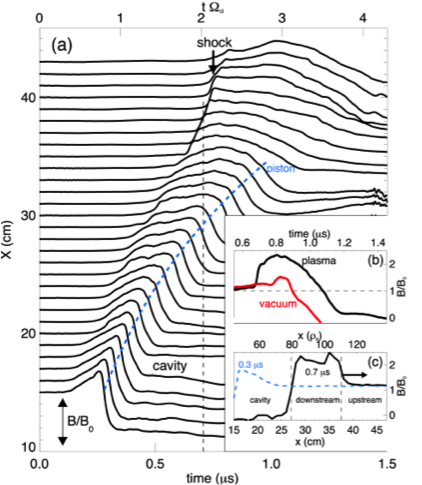
\includegraphics[width=3.0truein]{shock1}}
\caption{a) Magnetic stack plots of $B_{z}$ as a function of time for
  various distances from the target. (b) Comparison of $B_z(t)$ at $x
  = 35$cm with (black) and without (red) the ambient plasma. (c) Structure
  of the pulse before ($t = 0.3$ $\mu$s) and after a shock is formed.}\label{shock1}
\end{figure}

Figure~\ref{shock1}(a) shows stack plots of the measured magnetic field
$B_z/B_o$ for various
distances $x$ from the laser target. Each trace shows the typical
signature of a diamagnetic laser plasma cavity, including an initial
field compression followed by complete field expulsion. The magnetic
pulse ahead of the cavity travels at $370 \pm 20$ km/s, which is
super-Alfvénic ($M_A = 2.2 \pm 0.3$). The magnetic
piston, i.e., the leading edge of the diamagnetic cavity, slows from
500~km/s near the target to 200~km/s in the center of the vessel. About 20~cm from the target, corresponding to
$t \Omega_{i} =1$, the magnetosonic pulse starts to
steepen into a shock and to separate from the piston. The ramp continues
to steepen up to a distance of 40~cm from the target, at which point the
ambient plasma density drops sharply, and the shock dissipates. The
measured field compression of $B_z/B_o \ge 2$ is consistent
with the Rankine-Hugoniot jump conditions for a shock. In comparison
with expansion into vacuum (Figure~\ref{shock1}(b)), the field compression is
significantly larger with the ambient plasma and the leading edge of the
magnetic pulse expands faster, indicating that the pulse is carried by
ambient ions, which have been accelerated by the piston. Simultaneously,
the trailing edge of the pulse (i.e., the piston) moves much slower,
indicative of energy transfer to the ambient plasma. The magnetic pulse
in vacuum has a significantly shallower ramp due to fast ions that slip
through the magnetic field, causing a weak magnetic disturbance ahead of
the pulse. The spatial profile (Figure~\ref{shock1}(c)) shows a ramp with a width of
a few millimeters and a downstream region between the piston and the
ramp of 30 ambient ion gyroradii. In comparison to earlier times before
the shock is formed (blue dashed line in Figure~\ref{shock1}(c)), the structure of
the shock shows a significantly steeper and faster ramp, and a much
broader, more compressed pulse. In addition, the ramp of the shock
steepens from an initial 40 $c/\omega_{\rm pe}$ to less
than 20 $c/\omega_{\rm pe}$ at a distance of 40 cm from
the target. The measured shock formation time around
$t \Omega_{i} = 1$ is consistent with theoretical
predictions, while the measured coupling parameter of
$R_M/\rho_d = 1 \pm 0.1$ agrees
well with the requirements found in hybrid simulations~\cite{clark:2014}.

It should be noted that this result was enabled by the higher-density
plasma operation accessible with the new 20cm LaB$_6$ secondary
cathode added over the previous funding cycle.  Through increasing the
density in a core region by a factor of $\sim 10$ over the Barium
Oxide plasma source the ion skin depth was reduced and the formation
of the shock was successfully observed.

\subsubsection{Resonant interactions between energetic electrons and whistler
waves (J. Bortnik, R. Thorne, B. Van Compernolle; X. An (Graduate
Student) (UCLA))}


A major scientific problem of current interest is the determination of
the dominant physical processes that drive the dynamic variability of
the outer radiation belt \cite{thorne:2010, reeves:2013}. Resonant interactions between
energetic electrons and whistler mode waves are thought to play an
essential role~\cite{horne:2005, thorne:2013}. The ongoing theory-driven
LAPD project, led by J. Bortnik, has a two-pronged approach; the
resonant scattering of energetic electrons by whistler waves~\cite{vancompernolle:2014} is studied as well as the excitation of
whistler waves by energetic electrons. The experimental work has been
made possible by the development of a 10 cm diameter energetic electron
beam source, with beam energies up to 5 keV.

\begin{figure}[!htbp]
\centerline{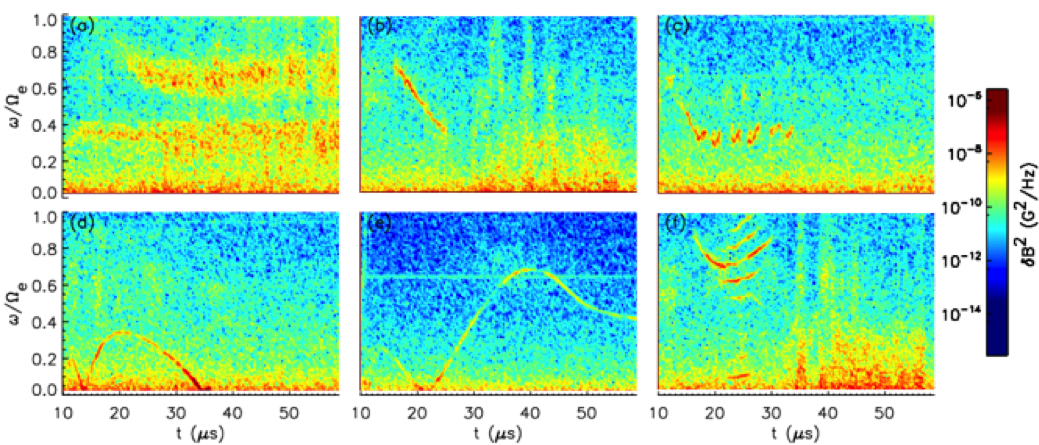
\includegraphics[width=5.0truein]{bortnik1}}
\caption{Examples of spectrograms of whistler wave excitation. (a)
  broadband waves, (b) falling tone, (c) multiple consecutive chirps,
  (d) double hook, (e) long rising and falling tone, (f) chirps at
  multiple frequencies simultaneously}\label{bortnik1}
\end{figure}


In the past two years the experiment has focused on the excitation of
whistler waves by energetic electrons under various plasma and beam
conditions. A very recent result~\cite{vancompernolle:2015a} is the excitation
of discrete frequency chirping whistler waves, which have been observed
in space for decades known as chorus waves, but have up to now never
been observed in the laboratory. The experiment identifies stringent
conditions under which the discrete frequency chirping is seen. There is
a strong dependence on beam density, plasma density and the guide field
profile and magnitude. Examples of the rich variety of beam-generated
wave activity is displayed in the spectrograms in Fig.~\ref{bortnik1}. The
experiment allows, for the first time, to test under controlled
conditions the leading theories in nonlinear whistler wave excitation.
Manuscripts are also being prepared on the excitation of broadband
whistler waves (non-chirping). It is shown that energetic electrons
resonantly excite whistler waves simultaneously through the Doppler
shifted cyclotron resonance, the Cherenkov resonance as well as through
the anomalous cyclotron resonance, i.e. through the relation $\omega -
k_\parallel v_{{\rm beam}, \parallel} = n\Omega_{e}$ where
$n=1,0,-1$. Comparisons with
growth rate calculations show excellent agreement with the
experiment.  Graduate student Xin An will present an invited talk on
this work at the upcoming APS DPP meeting in Savannah, GA.

\subsubsection{Fast-ion Campaign (W. Heidbrink, R. McWilliams (UC Irvine), B.
Breizman (UT Austin), F. Jenko (MPI Garching/UCLA), S. Tripathi, S.
Vincena, T. Carter (UCLA))}

This campaign, led by Prof. W. Heidbrink (UCI), has been focused on the basic
physics of the interaction between energetic ions and collective modes
supported by a magnetized plasma. It is motivated in part by the need to
understand the complex behavior of alpha particles in a burning,
magnetically confined plasma.  Work in this area has made use of lower
current beams~\cite{zhang:2007}, allowing the study of test particle behavior, in
addition to an up-to 25keV, 5A intense ion beam~\cite{tripathi:2011}, allowing for the
study of beam excitation of waves.    Topics of research have included
the classical transport of energetic ions in a magnetized
plasma~\cite{zhao:2005}, Alfv\'en waves in a periodic
mirror~\cite{zhang:2008a}, Doppler-shifted cyclotron interaction of
fast ions with shear Alfv'en waves~\cite{zhang:2008b,zhang:2009}

A recent campaign highlight is the investigation of the interaction
between fast ions and drift-wave turbulence in LAPD.  Confinement of
fast ions is a critical issue in fusion experiments; reaching the
burning plasma state and ignition requires confining alpha particles
and allowing them to slow down and heat the fusion plasma. A key
question is whether or not turbulence, which leads to significant
degradation of confinement of thermal ions, can impact fast ion confinement.
Many measurements of fast ion transport in
tokamaks are consistent with classical collisional theory, with fast
ion diffusion rates far below those for thermal ions (which are
impacted by turbulence).  However some recent measurements in tokamaks
have indicated anomalously high diffusion of fast ions, in
contradiction with earlier measurements and theoretical expectations.
A widely accepted explanation for the low transport of fast ions is that
energetic ions phase average over the microturbulence structure
along its large gyro and drift orbits.

\begin{figure}[!htbp]
\centerline{
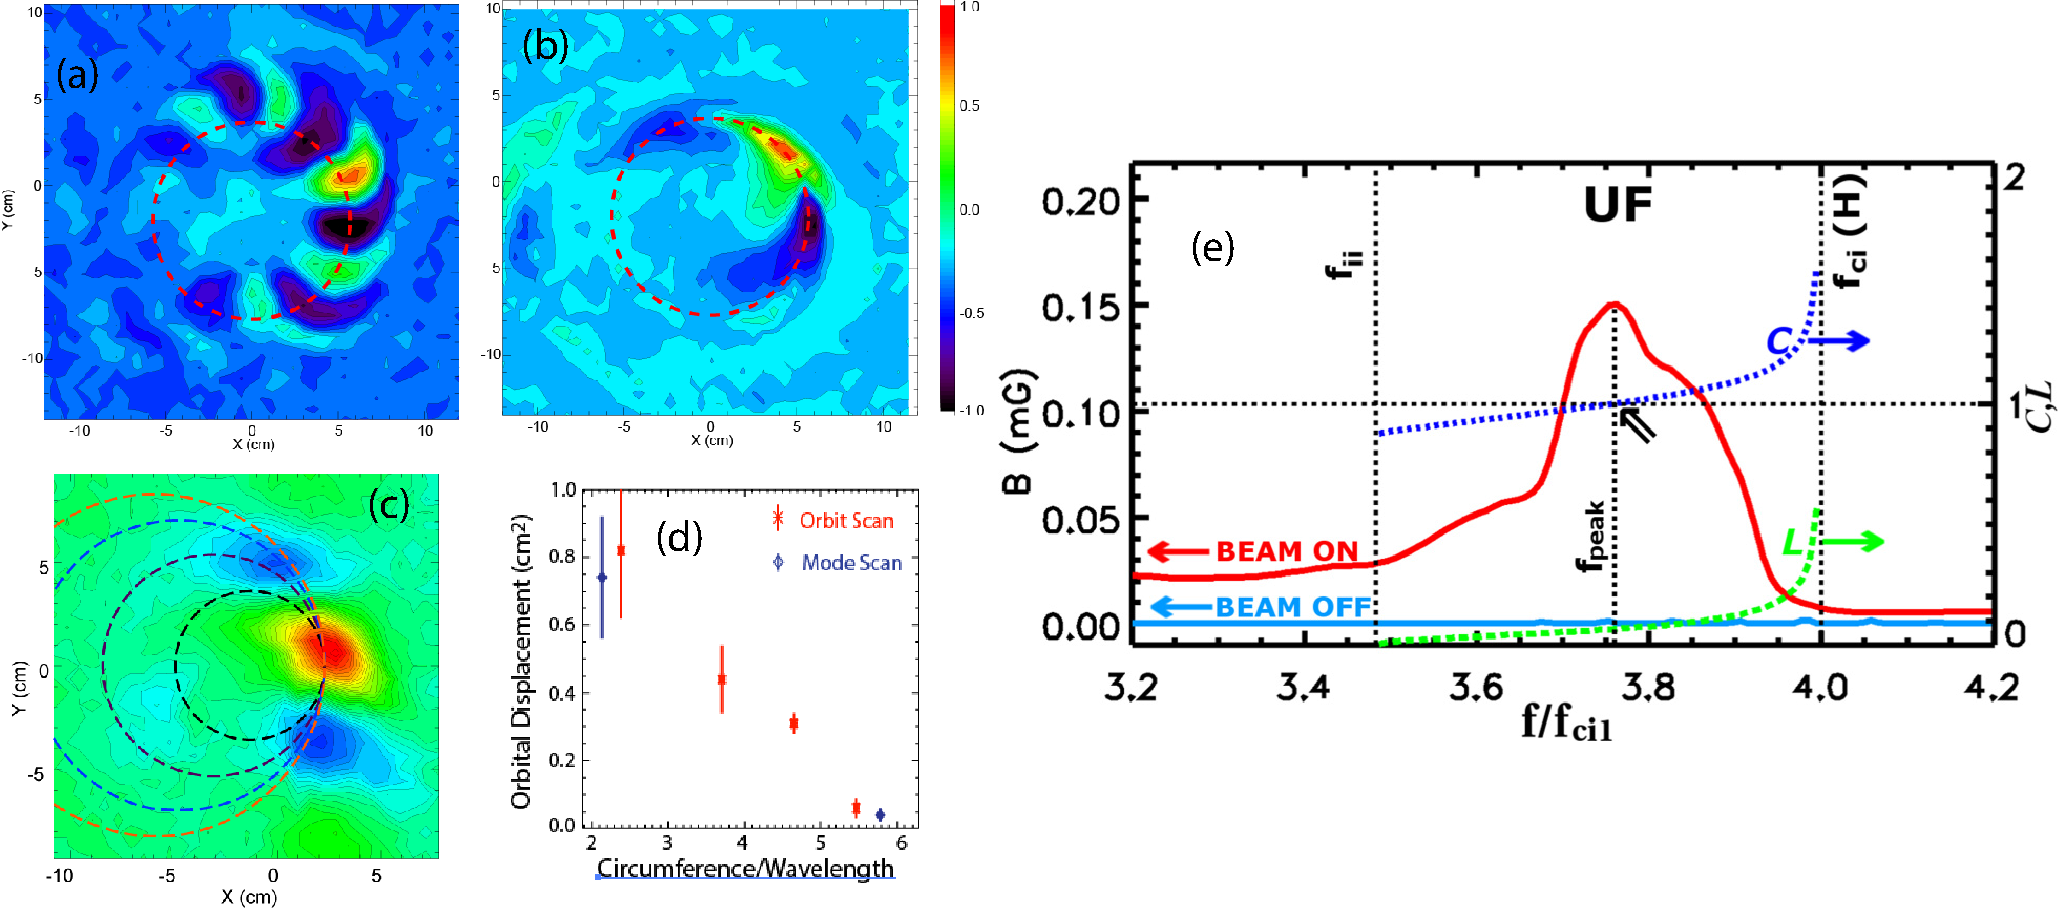
\includegraphics[width=3.5truein]{fastion}}
\caption{(a), (b), (c) Measured correlation function for electrostatic
  fluctuations in LAPD, with cartoon of ion orbit superposed. (d)
  Variation of orbital displacement with $\rho_{\rm
    fast}$/$\lambda_{\perp}$, where $\lambda_\perp$ is the
  perpendicular wavelength of the electrostatic fluctuations. }\label{fastion}
\end{figure}

An experiment performed in the
LAPD illustrates this fundamental
phase-averaging process~\cite{zhou:2010,zhou:2012a, zhou:2012b, heidbrink:2012}. A collimated, mono-energetic beam
of high-energy ions is launched in a uniform solenoidal field.
Obstacles are inserted into LAPD (either annular~\cite{zhou:2012a} or
planar~\cite{carter:2006}) in order to produce pressure gradients that drive
electrostatic fluctuations in the vicinity of the launched fast ion
orbits.  The ions traverse electrostatic fluctuations and their
deflected trajectories are measured.  The properties of the
electrostatic fluctuations, in particular the wavenumber and
correlation length, are varied through changing plasma properties, in
particular magnetic field.  

The response of the fast ions to the fluctuations is studied through
varying the dimensionless parameter $k_\perp \rho_{\rm fast}$, where
$k_\perp$ is the typical perpendicular wavenumber of the fluctuations
and $\rho_{\rm fast}$ is the gyroradius of the fast ions.  
In one version of the experiment (Fig.~\ref{fastion} (c)), the orbit size is varied
while keeping the spatial scale of the fluctuations fixed ; in another version (Fig.~\ref{fastion} (a),(b)), the
orbit size is held constant but the wave structure is varied.  In both
versions of the experiment, the orbital deflections are greatest when
the mode structure and orbit size are comparable (Fig.~\ref{fastion} (d)).  When
the wave field oscillates rapidly in space, the ion phase-averages the potential
fluctuations and is hardly deflected from its initial trajectory.
This effort was coordinated with research on the DIII-D tokamak~\cite{pace:2013} and
the toroidal basic plasma device TORPEX~\cite{heidbrink:2012,bovet:2012} and was key to establishing
that electrostatic fluctuations do not contribute substantially to the
transport of fast ions in fusion devices~\cite{pace:2013}.


\subsubsection{Alfv\'{e}n wave-wave interactions relevant to MHD turbulence (G.
Howes, F. Skiff, C. Kletzing (U. Iowa); T. Carter, S. Dorfman (UCLA))}

The unique capabilities of the Large Plasma Device (LAPD) have
contributed to our successful study of the fundamental nonlinear
interaction underlying astrophysical plasma turbulence, Alfven wave
collisions.  Early research on incompressible MHD turbulence in the
1960s \cite{Iroshnikov:1963,Kraichnan:1965} emphasized the wave-like
nature of turbulent motions in a magnetized plasma, suggesting that
nonlinear interactions between counterpropagating \Alfven waves---or
\Alfven wave collisions---mediate the turbulent cascade of energy from
large to small scales. A major goal of the turbulence community was to
demonstrate in the laboratory that this fundamental energy transfer
mechanism, derived in the limit of incompressible MHD, persists under
the realistic, weakly collisional plasma conditions relevant to many
astrophysical environments. The LAPD provided nearly ideal
experimental conditions for such an experiment, with sufficient size
to launch \Alfven waves from opposite ends of the plasma chamber and
unparalleled reproducibility to achieve a sufficient signal-to-noise
ratio to measure definitively the resulting nonlinear transfer of
energy to small scales.

\begin{figure}[!htbp]
\centerline{
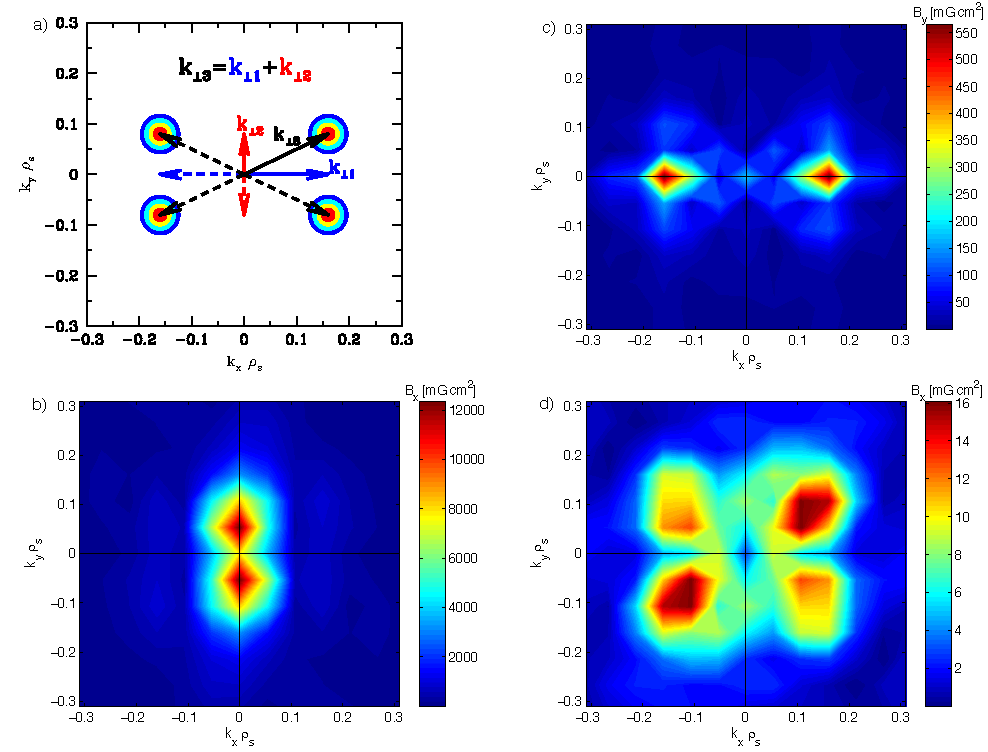
\includegraphics[width=3.5truein]{iowa}}
\caption{ (a) Diagram of $\V{k}_{\perp 1}$ for the ASW
antenna (blue) and  $\V{k}_{\perp 2}$ for the Loop antenna (red).
For the nonlinear daughter \Alfven wave, $\V{k}_{\perp 3}$ (black) is
the vector sum of the two antenna wave vectors, $\V{k}_{\perp 3} = +
\V{k}_{\perp 1} \pm \V{k}_{\perp 2} $ and $\V{k}_{\perp 3} = -
\V{k}_{\perp 1} \pm \V{k}_{\perp 2} $. Bullseyes indicate predicted
power distribution of the nonlinear product.  (b) Colormap (mG~cm$^2$)
of $\delta B_x(k_x,k_y)$ for the Loop antenna by itself.  (c) Colormap
of $\delta B_y(k_x,k_y)$ for the ASW antenna by itself. (d) Colormap
of $\delta B_x(k_x,k_y)$ for the nonlinear daughter \Alfven wave.}\label{iowa}
\end{figure}

This experiment was only possible through a collaboration that
employed specialized equipment built by plasma experimentalists at the
University of Iowa (UI) and UCLA and that followed an experimental
design relying on theoretical work at UI.  The experimental setup
involved the launching of one \Alfven wave using UI's Arbitrary
Spatial Waveform (ASW) antenna \citep{Thuecks:2009,Kletzing:2010} from
one end of the LAPD chamber, and another \Alfven wave using UCLA's
Loop antenna \citep{Auerbach:2011} from the other end. Theoretical
calculations of the nonlinear energy transfer in the weakly nonlinear
limit \cite{Howes:2013a}, along with validating gyrokinetic numerical
simulations \cite{Nielson:2013a}, guided a novel experimental design
\cite{Howes:2013b} that lead to the successful experimental
verification of the physics of \Alfven wave collisions in the
laboratory \cite{Howes:2012b,Drake:2013}, depicted in Figure~\ref{iowa}. The
theory predicts that the nonlinearly produced daughter \Alfven wave
will contain power in Fourier space arising from all possible sums and
differences of the Fourier power in the (b) Loop antenna wave and (c)
ASW antenna wave, as shown by the four bullseye pattern shown in panel
(a). The key experimental result (d) shows clearly this observational
signature of the nonlinear daughter \Alfven wave.  This result
demonstrates that the experiment successfully measured, for the first
time, the nonlinear interaction between counterpropagating \Alfven
waves, the fundamental building block of astrophysical plasma
turbulence.



\subsubsection{Radiation Belt Remediation (Campaign) (Dennis Papadopoulos, Tom
Antonsen (Univ. Maryland), Yuhou Wang, W. Gekelman, P. Pribyl, G.
Morales (UCLA))}

Laboratory observations of enhanced loss of magnetic mirror trapped fast
electrons irradiated by a shear Alfv\'{e}n Wave (SAW) are reported. A
trapped energetic electron population ($> 100$keV) is
generated in a magnetic mirror section (mirror ratio $\approx$ 2,
length = 3.5m) by an X-mode high power microwave pulse, and forms a hot electron
ring due to the grad-B and curvature drift. SAWs of arbitrary
polarization are launched externally by a Rotating Magnetic Field (RMF)
source ($\delta B/B_o \approx 0.1$\%, $\lambda_\parallel \approx 9$m).
Irradiated by a right-handed circularly polarized SAW, the loss of
electrons, in both the radial and the axial direction of the mirror
field, is significantly enhanced and is modulated at
f\textsubscript{Alfv\'{e}n}. The periodical loss continues even after the
termination of the SAW. Experimental observations suggest that a spatial
distortion of the ring is formed in the SAW field and creates a
collective mode of the hot electron population that degrades its
confinement and leads to electron loss from the magnetic mirror.

The hot electron ring was produced using a magnetron ($f=2.45$ GHz)
coupled to the plasma with a circular waveguide. The microwaves were
resonant with electrons at the second cyclotron harmonic (400G  near
the center of the magnetic mirror). A shear Alfv\'{e}n wave launched with a
rotating magnetic field antenna (located outside of the mirror)
de-trapped all electrons in a wide energy range (100 eV \textless{}
E\textless{}3 MeV). Evidence of SAW effectively de-trapping the hot
electron population is found in the x-ray flux measurement when the
trapped electrons are further accelerated to energies that enable hard
x-ray production~\cite{wang:2012}. Shown in Fig.~\ref{muri1} are
traces E-J, showing  that a burst of x-rays
generated by hot electrons escaping the mirror trap and striking
metallic surfaces appears during the Alfv\'{e}n wave propagation time. A
large flux of x-ray appears while the Alfv\'{e}n wave is first turned on.
After this initial burst, the x-ray flux decreases as the remaining hot
electron population is depleted during the rest of the Alfv\'{e}n on time.
After the Alfv\'{e}n wave is turned off, the x-ray flux slowly builds up due
to the presence of ECRH which remains on until $t = 30$ ms.

\begin{figure}[!htbp]
\centerline{
\includegraphics[width=3.5truein]{muri1}}
\caption{Time series of x-ray flux
measured by an un-collimated detector, designated by letters A-T. The
ECRH is on from t=0 to 30 ms, but only after about 20 ms are there
sufficient high energy electrons to produce a measurable x-ray flux.
Trace A is measured without launching the SAW. In traces B-T a 100 cycle
shear Alfvén wave pulse (total duration = 0.87 ms), starting at
different times labeled on the graph is launched. Each trace is averaged
over 50 plasma shots.}\label{muri1}
\end{figure}

After the ECRH terminates at $t = 30$ ms, a population of fast electrons
persists in the mirror, and can be de-trapped by launching Alfvén waves
at these late times, as evidenced by x-ray bursts in Fig.~\ref{muri1} traces K-T.
The estimated trapping time for a 200~keV electron is 40~ms before its
loss from cumulative collisions with the helium atoms and ions. The
decay of the x-ray burst intensity after $t = 31$~ms reflects the decay of
the number of x-ray producing hot electrons still in the mirror. This
measurement proves that the electron loss due to the shear Alfvén wave
is not related to the presence of the microwaves. An X ray tomography
system was developed to establish here the hot electrons go after having
interacted with the wave~\cite{wang:2013}. Most of the fast electrons strike the
waveguide, which is very close to the plasma edge. Electrons are also
lost of a mesh anode at the end of the device. These have been scattered
out of the loss cone~\cite{wang:2014}.




\subsection{Local group research}

\subsubsection{From heat transport in LAPD to chaotic fluctuations in DIII-D (J.
Maggs, G. Morales)}

An unexpected research path has lead to a connection between basic heat
transport experiments in LAPD to the identification that the density
fluctuations in the L-mode plasmas in the DIII-D tokamak are chaotic. To
simplify the study of electron heat transport, a series of basic
experiments have been performed in LAPD. The generic experiment uses a
small (3mm diameter), single-crystal LaB\textsubscript{6} cathode to
inject a low-voltage electron beam into a strongly magnetized (1 kG),
cold, afterglow-plasma. The low-voltage beam acts as an ideal heat
source that produces a long ($\sim$8 m), narrow ($\sim$5mm in radius) temperature
filament that is well separated from the walls of the machine. The
existence of a transition from a regime of classical transport to one of
anomalous transport has been established through detailed measurements.
During the period of classical transport, drift-Alfvén waves grow
linearly, driven by the temperature gradient. To elucidate the dynamics
leading to anomalous transport the permutation entropy analysis (C-H
plane technique) developed by \citep{rosso:2007} is applied to the
probe signals. This technique is an effective method to identify the
various possible dynamical processes (coherent, stochastic, chaotic,
fractional Brownian motion). In a characteristic C-H display, the
vertical axis corresponds to the Jensen-Shannon complexity, C, and the
horizontal axis to the normalized Shannon entropy, H. These quantities
are obtained from the Bandt-Pompe probability distribution~\cite{bandt:2002}
generated from the time series. Through these techniques it has been
conclusively shown that the LAPD anomalous heat transport is a
consequence of chaotic dynamics~\cite{pace:2008,maggs:2012a,maggs:2012b,maggs:2013}. Motivated by this finding a
collaboration was established with Dr. T. Rhodes who performs very
delicate Doppler-backscattering (DBS) measurements of the fluctuations
in the DIII-D tokamak. The analysis methodology developed for the LAPD
was applied to the DIII-D and it was found that the behavior of the
fluctuations in that seemingly different experiment exhibit the same
chaotic behavior as the simple LAPD experiment~\cite{maggs:2015}.

\begin{figure}[!htbp]
\centerline{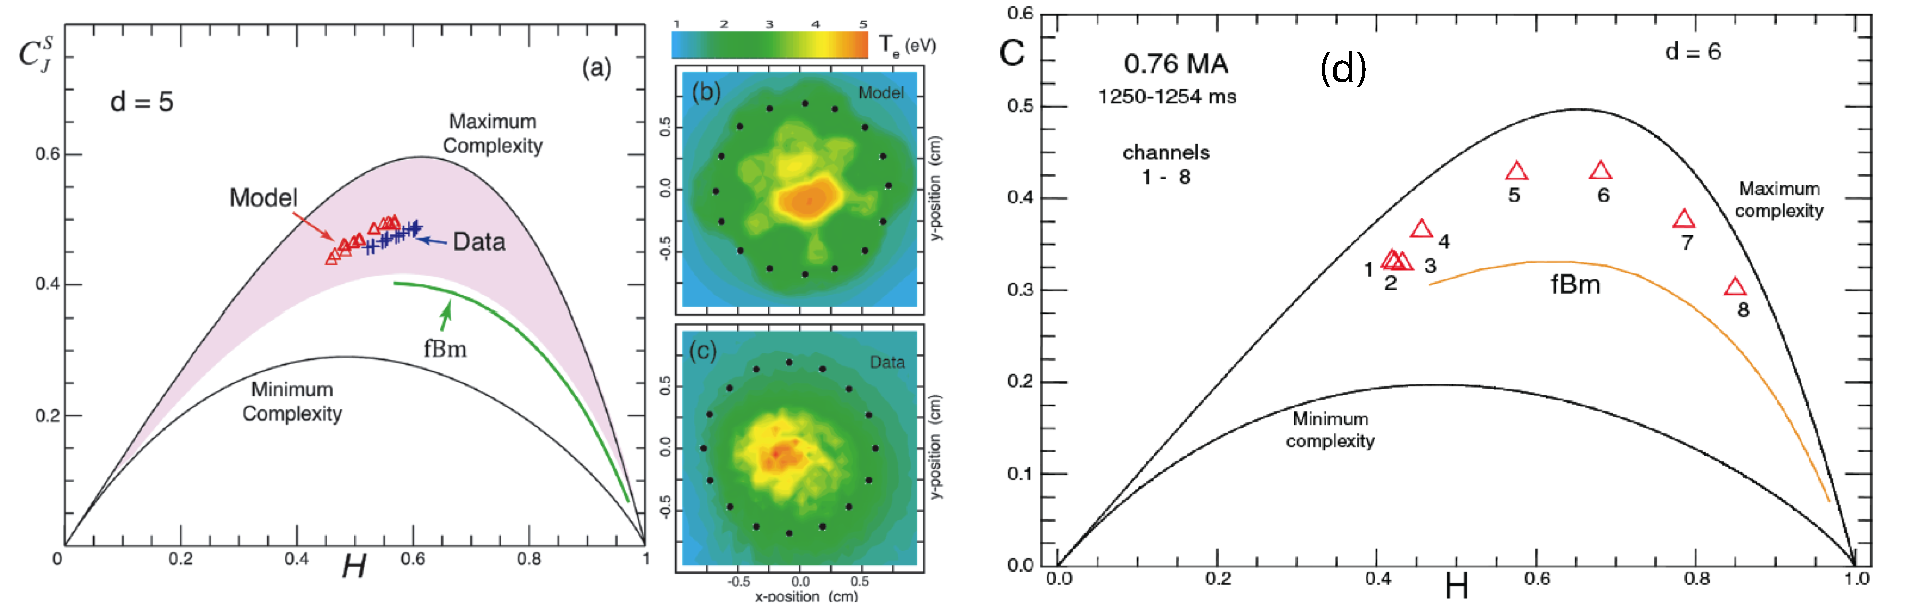
\includegraphics[width=6.0truein]{chaos}}
\caption{(a-c) C-H plane analysis of data in LAPD experiment and of prediction
of a chaotic advection model shows LAPD dynamics are chaotic. (d) C-H plane analysis of Doppler-backscattering (DBS) from DIII-D
shows that the signals from all the channels (different radii) are in
the chaotic region, as in the LAPD experiment. }\label{chaos}
\end{figure}


\subsubsection{Ion-ion hybrid Alfvén wave resonator (S. Vincena, G. Morales, J.
Maggs)}

A detailed experimental and theoretical investigation has firmly
established the reality of a wave resonator based on the concept of
wave reflection along the confinement magnetic field at a spatial
location where the wave frequency matches the local value of the
ion-ion hybrid
frequency~\cite{vincena:2010,vincena:2011,farmer:2012,vincena:2013,farmer:2013}. Such
a situation can be realized by shear Alfvén waves in a magnetized
plasma with two ion species because this mode has zero parallel group
velocity and experiences a cut-off at the ion-ion hybrid
frequency. Since the ion-ion hybrid frequency is proportional to the
magnetic field, in the presence of a magnetic well a wave resonator
can be formed. This is a structure that arises naturally in planetary
magnetospheres, and has relevance to mirror and tokamak fusion devices
because they must operate with a D-T mix, and their confinement fields
have axial gradients. A series of experiments were performed in LAPD
which started with the basic measurement of the properties of shear
Alfvén waves in the presence of two ion species in a uniform plasma.
Then it was established that the waves experience a cut-off when
propagating into a magnetic ramp, and finally a plasma with a magnetic
well in the center region of LAPD was explored. This led to the
conclusive identification of resonator behavior in a laboratory
environment when an external current loop excited trapped modes, both
in a pulsed and continuous operation.


\begin{figure}[!htbp]
\centerline{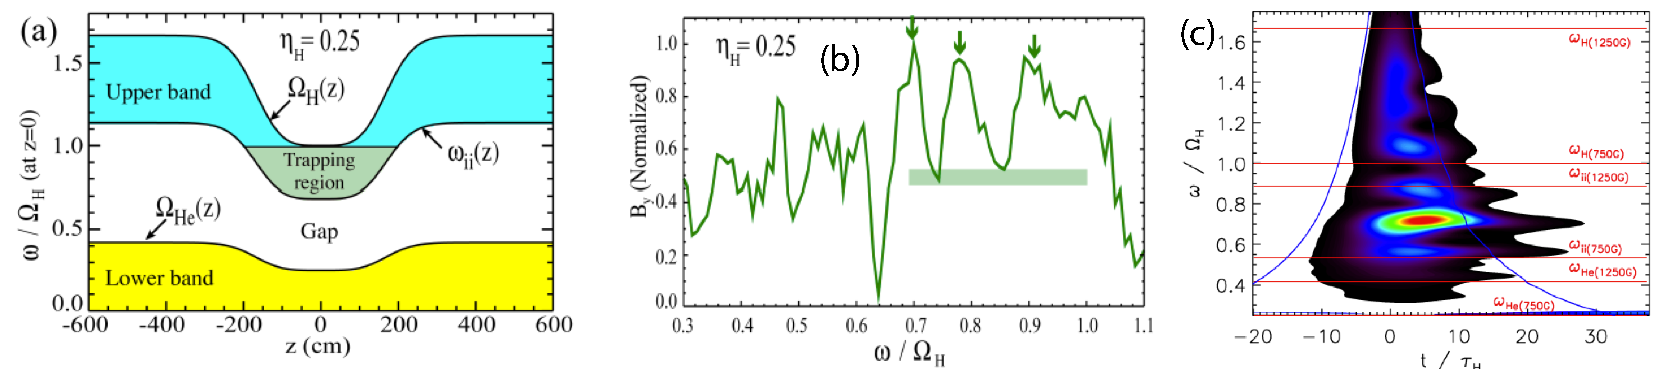
\includegraphics[width=6.2truein]{twoion}}
\caption{(a) Axial variation of resonator in LAPD for a
H-He\textsuperscript{+} plasma showing propagation bands and gap. (b)
Spectrum of magnetic fluctuations inside resonator shows resonator
peaks; arrows are theoretically-predicted frequencies of trapped
modes. (c) Contours of Morlet wavelet amplitude of magnetic field
fluctuations show the response of the
H\textsuperscript{+}-He\textsuperscript{+} resonator after excitation
with a current impulse of width $\Delta t = \tau_H$ at
$t = 0$. Red spot shows a large response and long lifetime of a
trapped mode.}\label{twoion}
\end{figure}

This work lead to a Ph.D. dissertation by W. Farmer and has been
reported in seven publications. The most recent effort has used the
insight from the LAPD studies to assess the properties of such a
resonator for the expected ITER environment and its excitation by
energetic alpha particles~\cite{farmer:2014}.


\subsubsection{Magnetic Flux Ropes (W. Gekelman, B. Van Compernolle; E.
Lawrence, T. DeHaas, D. Hong (Graduate Students))}

The UCLA group (W. Gekelman, B. Van Compernolle, and graduate students
past (Eric Lawrence) and present (Tim DeHaas, Dooran Hong) have done
groundbreaking work on the interaction of magnetic flux ropes. We are
presently collaborating with W. Daughton (LANL) on a experiment
dedicated to the memory of Tom Intrator.

The first ever experimental
determination~\cite{lawrence:2009} of a quasi-seperatrix layer
(QSL) was made on the LAPD in 2009. A QSL is a 3D region in which
magnetic field lines that start close to one another diverge rapidly in
space. The value of Q is a measure of the divergence. If two field lines
pass through a reconnection region, one or more components of B can
rapidly change within it leading to a large value of Q. This is
illustrated in Figure~\ref{ropes}.

\begin{figure}[!htbp]
\centerline{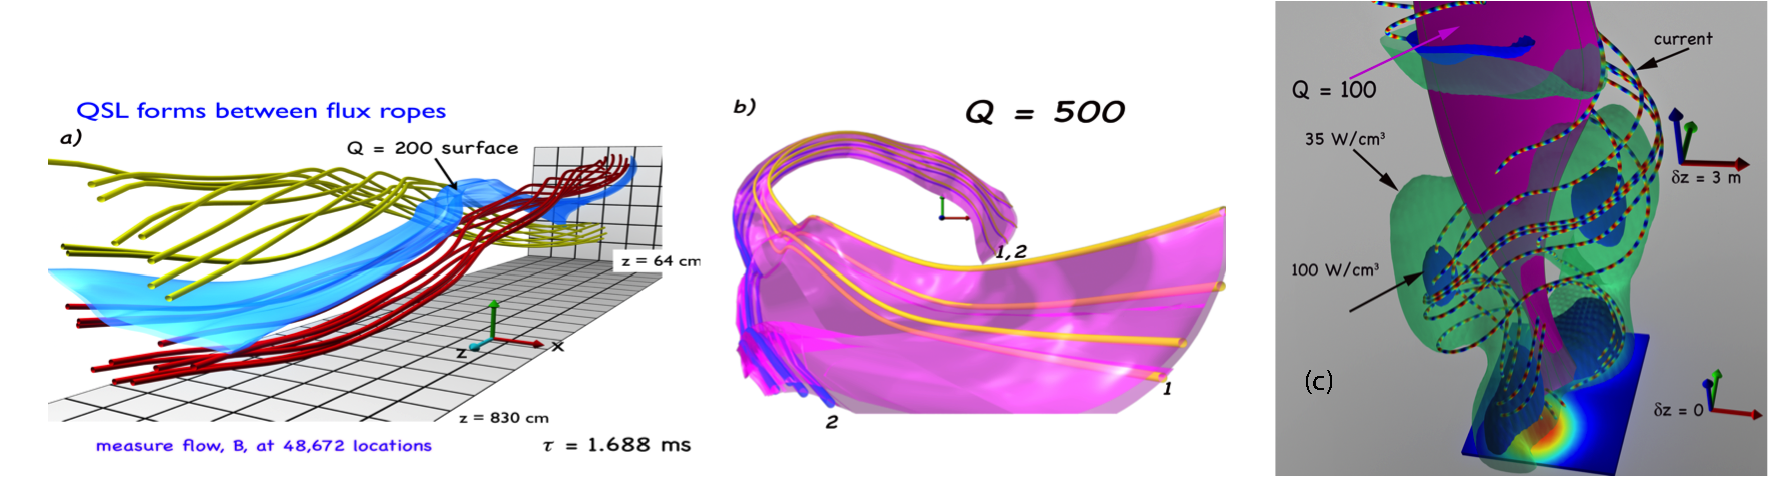
\includegraphics[width=6.2truein]{ropes}}
\caption{(a) The ``blue'' surface is a QSL (Q=100) which is located
between two flux ropes which are colored red and yellow. The flux ropes
are calculated by following field lines through the dense grid of
measurement points. (b) A Q=500 surface with several field lines
within it. One set of field lines labeled (1,2) are initially 0.5 mm
apart but are 12.5 cm apart when they reach the end of the measurement
volume 8.3 meters away. (c) Bottom is the plasma current in a plane 64 cm from the origin
of the ropes. The current of one rope is clearly visible and the current
density in the center is 5A/cm\textsuperscript{2}. A QSL of 100 is shown
along with several current field lines colored in stripes. Two
isosurfaces of the heating power are shown. Heating is observed within
the QSL at locations where reconnection occurs but significant heating
also occurs within the flux tubes.}\label{ropes}
\end{figure}

QSLs have been observed in the collision of two or more flux
ropes~\cite{gekelman:2010,vancompernolle:2011}. In a separate tearing mode experiment QSL's
were discovered when 3D current systems expanded in space and no field
line reconnection was involved. For the first time the total electric
field was measured using a
combination of magnetic and emissive probes. The parallel resistivity,
$\eta_\parallel$ was derived from the data and can
be 100's of times the Spitzer resistivity in small regions of space
during the collision of flux ropes. The resistivity was localized to the
gradients in the current of the flux ropes and also within the QSL.
Figure~\ref{ropes}(c) shows the QSL, current and $\eta_\parallel$
evaluated from the measured plasma current and electric field.
It is clear that there is more than one process at work. The three
dimensional case is very different from the traditional 2D models which
cannot predict the reconnection rate we measured by integrating the
electric field along magnetic field lines.

We have also studied chaos associated with the ropes and
found that it peaks when the flux ropes exist along with shear Alfvén
waves~\cite{gekelman:2014}. When the BaO cathode is replaced with a LaB\textsubscript{6}
cathode we will be able to do these experiments are relatively high
plasma beta and Lundquist number
(10\textsuperscript{5} \textless{} L \textless{}10\textsuperscript{6}).
How do intense Alfvén waves interact with flux ropes (which can also be
thought of as Alfvén waves)? What is the mechanism for this interaction
and can it lead to magnetic turbulence? The LAPD is the only machine in
which these experiments can be performed.

\subsection{Turbulence, transport and flows in LAPD (T. Carter, J. Maggs, P.
Popovich (UCLA) M. Umansky (LLNL), B. Dudson (U. York); D. Schaffner, B.
Friedman, G. Rossi (grad students))}

Suppression of turbulent transport by sheared flow has been
documented in a range of experiments and simulations~\cite{terry:2000}.  However we
still lack a complete, quantitatively correct theoretical model of
transport suppression by sheared flow.  This theoretical understanding
is essential in the development of a predictive capability for
turbulent transport, a capability that is critical in ensuring the
success of future experiments such as ITER. Experiments performed on LAPD have
documented in detail the response of turbulence and turbulent transport to
externally-controlled flow and flow shear.  

Azimuthal flow is driven in LAPD through biasing either the vacuum
chamber wall or an annular limiter relative to the plasma source
cathode.  Cross-field currents are driven (carried by ions due to
Pedersen conductivity), leading to $\mathbf j \times \mathbf B$ torque
and azimuthal rotation.  In the case of biasing the vacuum chamber
wall, H-mode-like behavior is observed, with suppression of turbulent
particle transport and steepening of the edge density
profile~\cite{maggs:2007,carter:2009}.  Transport is reduced from
Bohm-like levels to classical if the wall bias is above a threshold value (a factor of
~100 reduction in particle diffusion coefficient)~\cite{maggs:2007}.
%The threshold bias for confinement transition appears to be set by
%radial penetration of the driven azimuthal flow:  below the threshold,
%little to no flow and flow shear exists in the pressure gradient
%region (it is confined to a layer near the wall) and above the
%threshold, very large flow and flow shear penetrates into the gradient
%region, leading to the confinement transition.

A more detailed examination of the impact of flow shear on turbulent
transport was enabled through the introduction of an annular limiter
which brings a biasable surface closer to the plasma edge.  Biasing
the limiter relative to the cathode provides the ability to vary the
edge flow and flow shear continuously.  As the LAPD plasma
spontaneously rotates in the ion diamagnetic direction and biasing
tends to drive flow in the electron diamagnetic direction, zero shear
and zero flow states are accessible as well as flow reversal.
Figure~\ref{rotation}(a,b) shows the measured density gradient scale
length and turbulent particle flux as the flow shear is varied
continuously in the edge of LAPD.  The density gradient steepens
($L_n$ decreases) as shear is increased, indicating a reduction in
cross-field transport.  Consistent with this, the measured turbulent
particle flux drops monotonically with increasing shear~\cite{schaffner:2012}.  The shearing
rate on the $x$-axis is normalized to the turbulent autocorrlelation
time, as measured with zero flow shear; this is taken as a proxy for
the eddy decorrelation (or ``turn-over'') time.  Substantial changes
in both $L_n$ and particle flux occur for normalized shearing rates
of order unity.

\begin{figure}[!htbp]
\centerline{
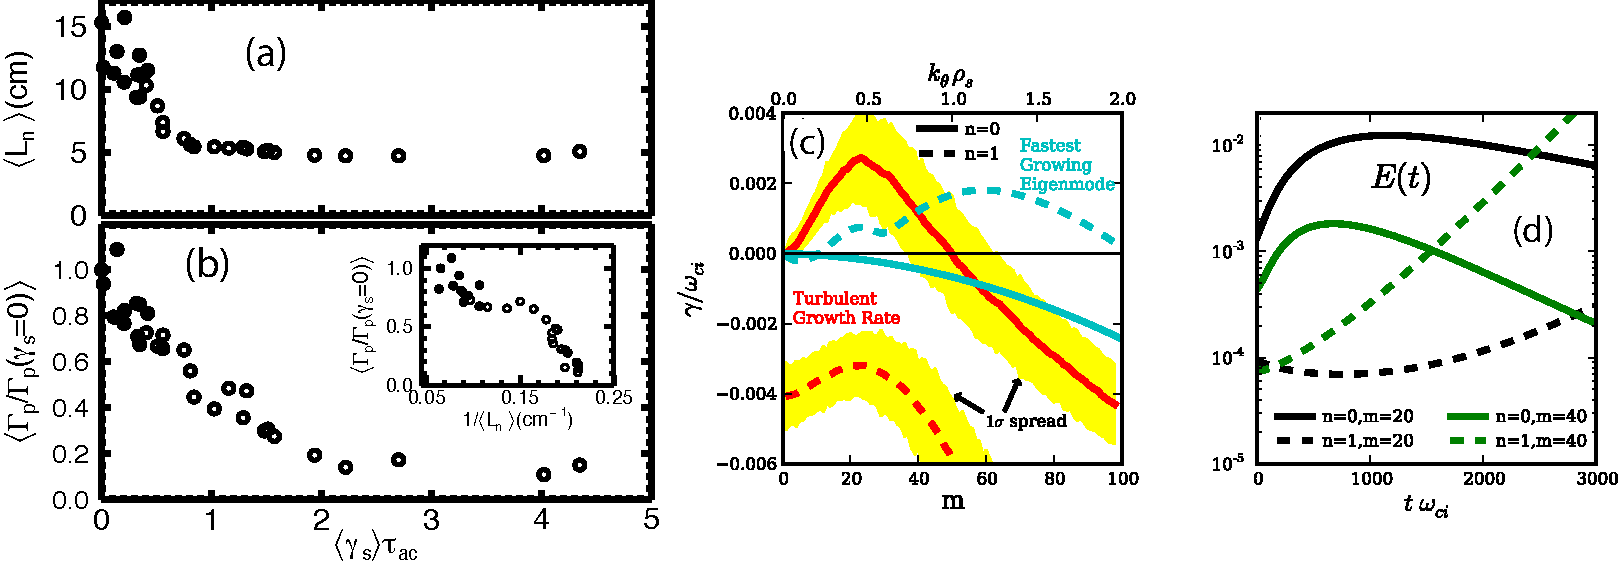
\includegraphics[width=6.2truein]{rotation}}
\caption{\label{rotation} (a)Gradient scale length versus shearing rate. (b)Particle flux normalized to no-shear
  flux as a function of normalized shearing rate. Filled symbols
  represent points with flow in the ion diamagnetic direction. Inset: Measured turbulent particle flux versus
  gradient scale length. (c) Linear evolution of energy starting from a turbu-
lent initial state. The $n = 0$ curves have an initial period
of transient growth before exponentially decaying. (d) Lin-
ear and turbulent growth rate spectra for $n = 0$ (solid lines)
and $n = 1$ (dashed lines) Fourier components. The linear
growth rates are those of the least stable eigenmodes, while
the turbulent growth rates represent the time rate of change of the
mode energy divided by twice the mode energy from the 
linear simulation. The shaded region marks the $1\sigma$ spread in the
turbulent spectrum, obtained from the distribution of growth rates in
the nonlinear simulation.
}
\end{figure}


LAPD experimental data has been compared to a number of analytical theoretical models of shear
suppression~\cite{schaffner:2013}.   The ability to continuously vary
the edge flow shear in LAPD allowed the collection of data for both
the weak ($\gamma_s \tau_{\rm ac} < 1$) and strong ($\gamma_s
\tau_{\rm ac} > 1$) shearing regimes.  The data was fit to two
functional forms motivated by theoretical models developed for these
two regimes.  While these functional forms do fit the data reasonably
well, the fit coefficients obtained are not a good match to
theoretical predictions, suggesting that new models may be needed to
explain LAPD data.  Future work will focus on comparison of LAPD data
to numerical simulation (e.g. using the GENE code) and to more
recently developed analytical models of shear suppression of turbulent
transport~\cite{staebler:2013}.

Turbulence in magnetically confined plasmas is often attributed to
linear instabilities, which can grow from infinitesimal initial
perturbations (e.g. thermal noise). However, it is well known in the
hydrodynamics community that linear instability (normal mode) analysis
fails at predicting turbulent onset for a number of physical
situations, for example water flow in cylindrical pipes (Poiseuille
flow). In these cases, turbulence arises even though all linear modes
are stable, meaning infinitesimal perturbations on the laminar state
cannot grow exponentially. Nevertheless, finite amplitude
perturbations can still excite turbulence. We have found that the same
can be true in pressure-gradient-driven turbulence in LAPD.
Simulations of LAPD turbulence have been performed using the BOUT++
code, which has been modified for
LAPD geometry and boundary
conditions~\cite{popovich:2010a,popovich:2010b,umansky:2011,friedman:2012a}.  Even though the
resistive drift-Alfv\'{e}n wave is linearly unstable, the simulations reveal that a
nonlinear instability controls the saturated turbulent state~\cite{friedman:2012b,friedman:2013,friedman:2014,friedman:2015},
as shown in Figure~\ref{rotation}(c).  Consistent with this observation, transient growth of linearly-stable
flute-like ($k_\parallel = 0$) modes is observed, as shown in
Figure~\ref{rotation}(d).  


A similar conclusion was previously reached by authors examining
tokamak edge turbulence simulations~\cite{drake:1995, biskamp:1995,
scott:1990}.  The dominance of a nonlinear instability makes prediction
of turbulence and turbulent transport in magnetic confinement
experiments difficult as linear instability calculations, which are
relied on quite heavily in the fusion community, can be misleading.
Using input from analysis of BOUT++ simulations, a technique has been developed 
that enables the prediction of the nonlinear properties of a turbulent
system using simple linear, but ``nonmodal'', calculations. The
technique successfully predicts the structure of the nonlinearly
saturated state in LAPD turbulence simulations and provide a linear
technique to estimate turbulent saturated amplitude and particle
transport~\cite{friedman:2014,friedman:2015}.  

This work has resulted in two graduate students completing PhDs over
the last 5 year period (David Schaffner and Brett Friedman) and the
training of two postdoctoral fellows (Pavel Popovich and Brett
Friedman).  



\section{Facility Development: Cathode Upgrade}

Since its inception, the BaPSF has continually improved the capabilities
and diagnostics of the LAPD device. In the next funding period, among
other improvements, we propose one major upgrade to the LAPD. This
upgrade will replace the primary plasma source, currently a large-area
Barium Oxide emissive cathode, with a Lanthanum Hexaboride (LaB$_6$) based
cathode. Large area LaB6 cathodes have been developed over the last
funding period by the UCLA group (see the Appendix for more details) and
offer many advantages to BaO cathodes, including access to important new
parameter regimes and significant operational advantages.

LaB$_6$ cathodes offer far more emission current density, and
therefore higher density and temperature plasmas, than BaO cathodes.
Recently, a 20cm LaB$_6$ cathode has been installed on LAPD (see
Appendix), allowing for the production of high density and temperature
``core'' plasmas within the larger BaO-produced plasma. Plasmas are
produced with significantly higher density (up a factor of 50 from BaO
to $5\times 10^{13}$ cm$^{-3}$) and higher electron temperature (up to
$12-15$eV from $\sim 5$~eV with BaO); see Fig.~\ref{lab6}. At this
electron density and temperature, the ion-electron collisional energy
exchange time is calculated to be $\sim 0.2$~ms and, consistent with
this, an increased ion temperature is observed in the new LaB$_6$
produced plasma. Initial measurements of shape of the He II 468.6~nm
ion emission line have been performed using a 2m monochrometer. These
measurements have been compared to PrismSPECT Spectral Analysis Code
calculations yielding a best-fit temperature of $T_i \sim 6$~eV, a
significant enhancement over the BaO produced plasma ion temperature
of $T_i \lesssim 1$~eV (see Figure~\ref{lab6}(c)).
Table~\ref{lapdparams} gives a comparison of plasma parameters
achievable in the BaO and LaB$_6$ cathode plasmas.  There is some
flexibility in operating the LaB$_6$ source, in particular the
emissivity of the cathode can be controlled through raising or
lowering the temperature.  By lowering the temperature and the
emissivity, plasmas with parameters similar to BaO cathode plasmas can
be produced. Part of the local group research time would be dedicated
to developing operational regimes using a new LaB$_6$ plasma. In
particular, developing lower collisionality regimes is of interest.
Plasmas created so far using the smaller LaB$_6$ sources have similar
electron collisionality to BaO plasmas: the electron temperature is
higher, but the gains in collisionality are wiped out by increased
density.  The ion collisionality is lowered due to the substantial
increase in ion temperature in the new source.  It may be possible to
develop an operational condition where the plasma density is lowered
(perhaps similar to BaO plasmas) but with increased electron
temperature; developing this regime (perhaps using high temperature
cathode but with low fill pressure) will be a focus of future work by
the local group.  

\begin{figure}[!htbp]
\centerline{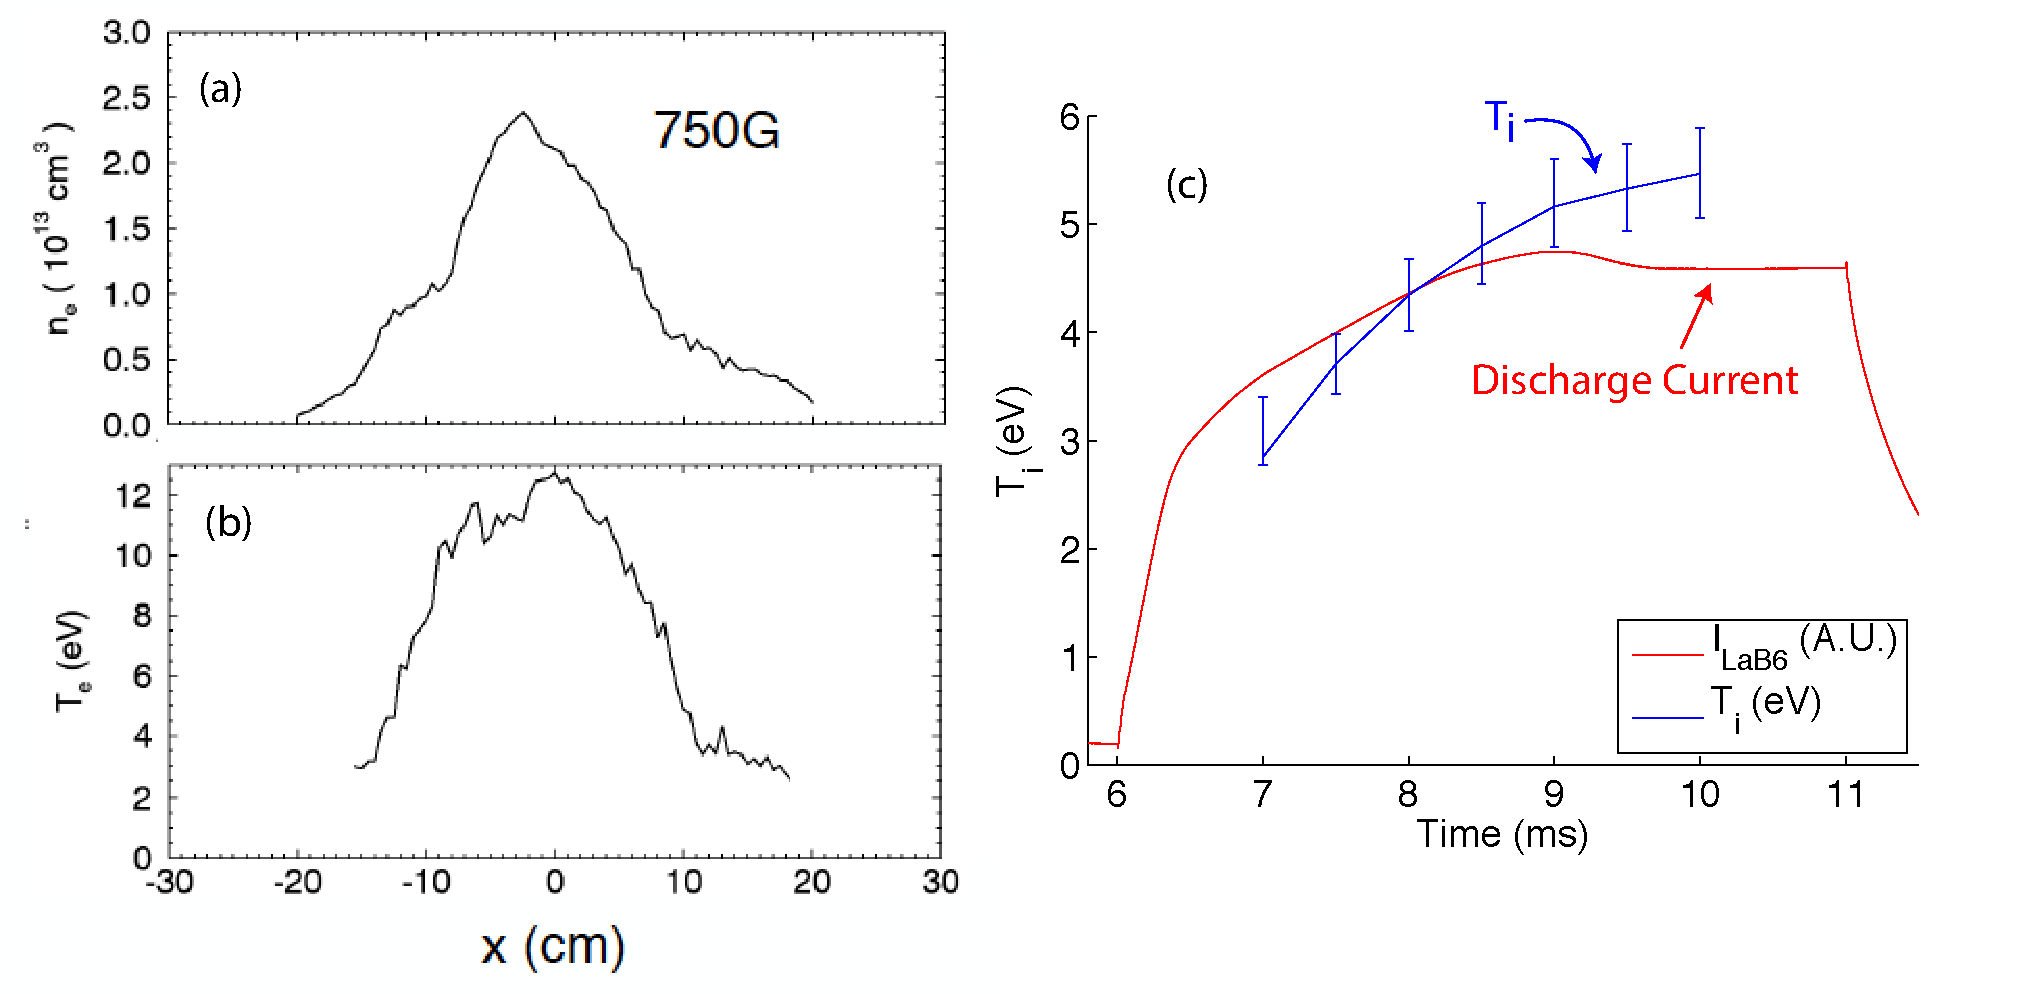
\includegraphics[width=6.0truein]{lab6}}
\caption{(a) Density and (b) Electron temperature profiles for plasmas
generated with the 20cm LaB$_6$ secondary cathode in LAPD. (c) Time
history of the LaB$_6$ cathode discharge current and ion temperature
(measured spectroscopically).}\label{lab6}
\end{figure}

\begin{table}[!htbp]
%\begin{wraptable}{R}{0pt}
{\begin{tabular}{|p{2.8truein}|c|c|c|c|}
\hline \hline
Parameter & BaO (1 kG) & LaB$_6$ (1 kG) & LaB$_6$ (400G) & LaB$_6$ (125G) \\ \hline
\hline
Density (cm$^{-3}$) & 2$\times 10^{12}$ & 2$\times 10^{13}$ & 2$\times 10^{13}$ & 2$\times 10^{13}$ \\\hline
Electron temperature (eV) & 5-10 & 6-15 & 6-15 & 6-15 \\\hline
Ion temperature (eV) & $<$1 & $\sim T_{\rm e}$ & $\sim T_{\rm e}$ & $\sim T_{\rm e}$ \\\hline
Electron gyroradius (mm) & 0.06 & 0.08 & 0.21 & 0.66 \\\hline
Ion gyroradius (cm) & 0.2 & 0.7 & 1.8  &  5.7 \\\hline
Ion sound gyroradius (cm) & 0.5 & 0.7 & 1.8 & 5.7 \\\hline
$c/\omega_{\rm pe}$ (mm) & 4 & 1 & 1 &1 \\\hline
$c/\omega_{\rm pi}$ (cm) & 50 & 15 & 15 & 15 \\\hline
Ion cyclotron frequency (kHz) & 380 & 380 & 152 & 48 \\\hline
Electron collision frequency (MHz) & 3 &  10 & 10 & 10 \\\hline
Ion collision frequency (kHz)  &  300 & 100 & 100 & 100 \\\hline
Typical Alfv\'{e}n wave frequency (kHz) & 200 & 200 & 100 & 25 \\\hline
Plasma Beta  & $4\times 10^{-4}$ & 1.6\% & 10\% & $\sim 1$ \\\hline
\hline
\end{tabular}}
\caption{Typical parameters for helium discharges in
  LAPD. }\label{lapdparams}
%\end{wraptable}
\end{table}

The parameters accessible using a LaB$_6$ source opens up a range of
possible new research directions using LAPD.  The higher density
reduces the ion skin depth scale to be smaller than the perpendicular
size of the plasma.  This fact allowed the first observation of a
magnetized collisionless shock in LAPD using the small LaB$_6$
secondary source~\cite{}.  The installation of a larger LaB$_6$ source
will allow further studies of the shock properties by allowing more room
for the shock to develop and evolve.  Studies of magnetic
reconnection and magnetic flux ropes have also been enabled by the
development of LaB$_6$ cathodes, including the study of the tearing of
a current sheet~\cite{}.  Future studies would make use of the larger
plasma source to generate longer current sheets for exploration of
reconnection and current sheet instabilities.  The increased
density also enables studies of compressional Alfv\'{e}n waves by
shortening their perpendicular wavelength to fit inside of LAPD.
Studies of fast wave physics will be the subject of local group
research as well as a new Campaign.  

LaB$_6$ cathode-produced plasmas provide the opportunity to study the
linear and nonlinear physics of Alfv\'{e}n waves in plasmas with $T_i
\sim T_e$ and at higher beta ($\beta \sim 1$ is possible through
reduced magnetic field).  With hot ions, finite ion Larmor radius
effects are expected to modify propagation of oblique Alfv\'{e}n
waves~\cite{hasegawa76,lysak96}.  With increased plasma beta (meaning
$v_{\rm A} \sim v_{\rm th,i}$), kinetic damping of Alfv\'{e}n waves
can be due to resonant interactions with ions: ion Landau damping due
to parallel electric fields in the wave or ion Barnes or Transit Time
Magnetic Pumping damping due to compressive fluctuations modifying the
background magnetic field~\cite{barnes66}.  The nature of nonlinear
interactions between Alfv\'{e}n waves is modified by increased ion
temperature and increased plasma beta; for example, ion sound waves
should be heavily damped with $T_{\rm i} \sim T_{\rm e}$, which
impacts parametric decay.  If ion temperature anisotropy can be driven
in LAPD (RF heating? Flow into an expanding magnetic field?), the
large acheivable $\beta$ may allow the study of 
instabilities such as the mirror~\cite{} and firehose~\cite{} which are known to be
important in the solar wind~\cite{bale} and may be important in other
astrophysical settings (such as in accretion disks~\cite{}).   This
new regime will be the subject of study by the local group as well as
external users, the new ``Solar Wind'' campaign (described below) will
leverage the new capabilities.

Operationally, Lab$_6$ cathodes are far more robust than BaO cathodes.
BaO cathodes are sensitive to Oxygen; any significant exposure to
Oxygen will ``poison'' the cathode, substantially lowering its
emission current. For this reason, any unintentional vacuum leak leads
to an extended shutdown: it takes around 10 days to replace a poisoned
cathode (cathode must be removed, cleaned, re-coated and slowly
``converted'' while heated under vacuum before it is ready to be
operated). In addition, the introduction of apparatus into the vacuum
chamber in order to perform experiments (e.g. probes or antennas) must
be done very carefully. New apparatus is pumped down to $5\times
10^{-6}$~Torr prior to being opened and inserted into the vacuum
chamber to prevent Oxygen from being introduced. For typical probes it
can take 2 hours to achieve this level of vacuum and it can take up to
a day of pumping for larger items (e.g. antennas, ion beams). The
efficiency of gathering data using LAPD is therefore reduced by time
waiting to open new probes (e.g.  after moving a probe to a new axial
location). LaB6 cathodes are far more robust and do not suffer from
the same sensitivity to vacuum incidents.  With a LaB$_6$ primary
cathode we anticipate that pumping probes into the $10^{-4}$~Torr
range will be sufficient before opening (this typically takes 10-15
minutes).  Using LaB6 for the primary LAPD cathode will therefore
significantly increase efficiency of data taking during the
typical run week. Overall uptime for the LAPD has been very good over
the past 5 year period, but would be significantly better with a
LaB$_6$ plasma source: for example, a prototype LaB$_6$ plasma source was operated at
1~Hz continuously for 1 year in the ETPD without need for a
maintenance opening. 

\begin{figure}[!htbp]
\centerline{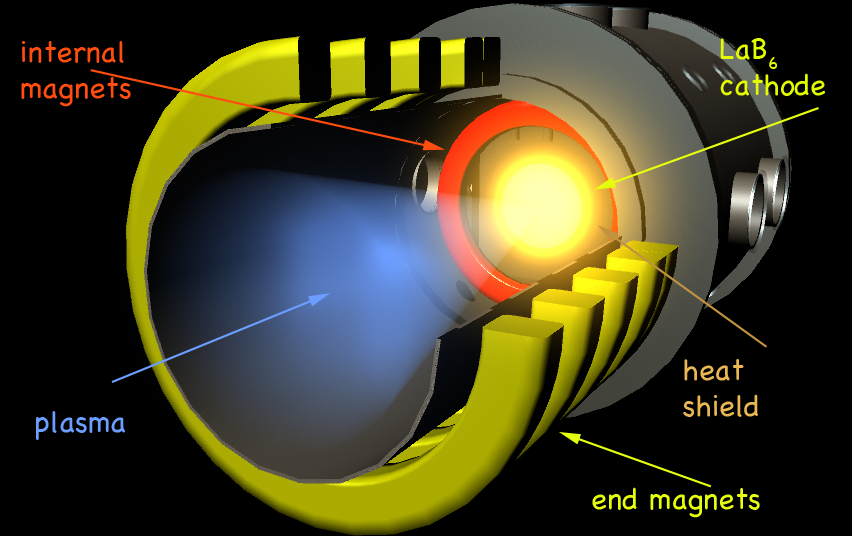
\includegraphics[width=4.0truein]{lab6-proposal}}
\caption{Conceptual design for new primary LaB$_6$ cathode source with
  internal magnets for LAPD}\label{newcath}
\end{figure}

A new LaB$_6$ cathode will be constructed as a permanent replacement
for the current 75cm BaO cathode.  Due to the significant power
required to heat LaB$_6$ to optimal emission temperature (1800C), it
is not practical to build a 75cm cathode.  Instead, a 40cm source will
be constructed based on the proven graphite heater and LaB$_6$ cathode
technology developed by the UCLA group.  This smaller source will then
be used to create a larger (60cm diameter) plasma through expansion of
the magnetic field from the source region into the main chamber.  An
internal (to the vacuum chamber) magnet will be fabricated to strongly
magnetize the source region (up to 8kG) in order to produce $\sim
60$cm diameter plasmas in the main chamber at nominal magnetic field
values (up to 2kG).  A rendering of the new plasma source is shown in
Fig.~\ref{newcath}.  Funding in the amount of \$600k has been
requested in the first year to purchase components for the new
cathode source, including internal magnets and power supplies for the
magnets and the new discharge source.  Construction  will be carried
out over the first two years of the new award, led by Assoc. Director
Prof. Gekelman.


\section{Proposed Research - Local Group}


\subsection{Research on Three Dimensional Current Systems and Magnetic Field
Line Reconnection (W. Gekelman, B. Van Compernolle)}

The UCLA group (W. Gekelman, B. Van Compernolle, graduate students and
external users: W. Daughton (LANL), will continue their successful
program on 3D reconnection. Much of the past work has centered on
reconnection in systems of magnetic flux ropes. The first ever
experimental determination~\cite{lawrence:2009} of a quasi-seperatrix
layer (QSL) was made on the LAPD in 2009. A QSL is a 3D region in
which magnetic field lines that start close to one another diverge
rapidly in space. The value of Q is a measure of the divergence.  If
two field lines pass through a reconnection region, one or more
components of B can rapidly change within it leading to a large value
of Q. This has been seen in the collision of two or more flux
ropes~\cite{gekelman:2010}. In a separate tearing mode experiment
QSL's were discovered when 3D current systems expanded in space and no
field line reconnection was involved. For the first time the total
electric field was measured using a combination of magnetic and
emissive probes. The parallel resistivity was derived from the data
and can be 100's of times the Spitzer resistivity in small regions of
space during the collision of flux ropes. The resistivity was
localized to the gradients in the current of the flux ropes and also
within the QSL. It is clear that there is more than one process at
work. The three dimensional case is very different from the
traditional 2D models which cannot predict the reconnection rate we
measured by integrating the electric field along magnetic field
lines. We have also studied chaos associated with the
ropes and found that it peaks when the
flux ropes exist along with shear Alfvén waves~\cite{gekelman:2014}.

We will continue to explore the nature of 3D current systems and
reconnection in future experiments. What are all the instabilities that
give rise to large plasma resistivity's. Are high frequency waves
involved? With the planned replacement of the BaO cathode we will be
able to do these experiments are relatively high plasma beta and Lundquist number
(10\textsuperscript{5} \textless{} L \textless{}10\textsuperscript{6}).
How do intense Alfvén waves interact with flux ropes (which can also be
thought of as Alfvén waves)? What is the mechanism for this interaction
and can it lead to magnetic turbulence? The LAPD is the only machine in
which these experiments can be done. We look forward to continued
collaboration with the Los Alamos group as well with others interested
in this topic.

\subsection{Avalanche phenomena in magnetized plasmas (B. Van Compernolle, G.
Morales)}

Avalanches are sudden events that cause major changes over an extended
region of a physical system. The origin of avalanches is the presence of
a steep gradient in one of the system parameters. Often there is a
threshold value for the gradient; when it is exceeded, a complex
sequence of processes is triggered whose role is to relax the gradient
below the threshold value. In several environments, such as an
externally-heated or fueled plasma, the sources reestablish the gradient
and further cause it to exceed the threshold value. A sequence of
avalanches can then occur, but the actual time of appearance of an
individual event displays a marked degree of unpredictability. The
behavior is intermittent and causes the parameters of the system to
evolve from place to place, i.e., there is an associated ``transport''
that occurs. It is this type of intermittent avalanche phenomena that
will form the central theme of the proposed studies.

The project will focus on avalanches triggered by gradients in plasma
temperature and density across the magnetic field. This is a situation
encountered in natural plasmas (e.g., sun, earth's magnetotail) and in
fusion devices. The technological breakthrough that makes possible the
implementation of an ideal basic configuration for studies of avalanches
in magnetized plasmas is a reliable and flexible LaB\textsubscript{6}
cathode source that has been developed in BaPSF.

Preliminary results demonstrating the controlled generation of
avalanches using a ring-shaped heat source have been recently
published~\cite{vancompernolle:2015b}. In the near future a full
characterization of cross-field avalanches will be made using the
diagnostic tools available at the LAPD laboratory. Detailed spatial
and temporal measurements of density, temperature, plasma potential,
flows (both ExB and diamagnetic), and magnetic fields, will be
undertaken for a wide range of parameter values, including: heating
power, strength of confinement magnetic field, neutral gas
fill-pressure and ionic species.. The steepness of the pressure
gradient can be adjusted by changing the heating power, which
determines the peak electron temperature within the hot ring. Although
the preliminary results were performed with a constant bias voltage
applied to the LaB\textsubscript{6} source, a straightforward
extension is to control, and change, the bias voltage during the
experiment. This capability permits the identification of various
features, such as hysteresis and response to modulations of the
critical gradient.

In summary, the wide range of experimental capabilities at BaPSF allows
for the investigation of a number of important questions related to
avalanches in magnetized plasmas including quantitative information about SOC dynamics, the formation and evolution
of streamers, the effects of flows, the connection between avalanches
and 'blobs', and the role of nonlocal transport of both temperature and
density during avalanche events.


\subsection{Turbulence and Transport (T.
Carter, S. Vincena)}

\subsubsection{Turbulence and Transport in increased $\beta$, warm ion plasmas} 

We propose to study the fundamental physics of
pressure-gradient-driven instabilities and associated turbulence and
transport in an experiment where the $\beta$ value can be varied over
several orders of magnitude, from $\beta\sim 10^{-4}$ to $\beta\sim
1$. In the near term, this work is enabled by the new secondary small
LaB6 plasma source; the new larger area $LaB_6$ plasma source that can
create plasmas with significantly increased thermal energy density,
which, along with the ability to vary the magnetic field while keeping
the plasma magnetized, allows for accessing a wide range of $\beta$
values. In addition, the production of warm ions provides an
opportunity to investigate ion kinetic effects on the turbulence. In
the proposed work, focus will be given to a detailed, quantitative
study of the response of turbulence, turbulent transport, and
spontaneously generated flows to variation of $\beta$. Existing
capabilities to externally control flow and flow shear will be used to
extend previous work on the suppression of particle transport by flow
shear to higher $\beta$ regimes. Finally, we will
undertake work to make a very important further development regarding
the capability to simulate LAPD plasmas, including kinetic
effects. The state-of-the-art gyrokinetic turbulence code GENE,
capable of handling high $\beta$ electromagnetic
effects, will be used for simulation studies of LAPD plasmas; this work
will be carried out in collaboration with Prof. F. Jenko (UCLA). These
will be the first global ab initio computations of LAPD plasmas,
allowing to carry out simulation-experiment comparisons in the high
$\beta$ regime with unprecedented quality.

\subsubsection{Turbulence and transport in multiple ion species
  plasmas} 

More needed here


\subsection{Physics of Compressional Alfven waves in LAPD (Vincena, Tripathi,
Van Compernolle)}

More needed here


\subsection{Linear and nonlinear properties of Alfv\'{e}n waves in
  increased $\beta$, warm ion plasmas (Carter, Gekelman, Van
  Compernolle, Vincena, Tripathi)}

The proposed research would seek to utilize new plasma parameters
provided by LaB$_6$ cathodes in LAPD to significantly extend past
studies on the linear and nonlinear physics of Alfv\'{e}n waves.


LAPD to: (1) Document the linear characteristics of Alfv\'{e}n waves
in warm ion, increased beta plasmas in LAPD, (2) Study the absorption
of high power Alfv\'{e}n waves on ions via Landau/Barnes damping and
cyclotron damping in a magnetic beach, and (3) Extend recent studies of
nonlinear beat-wave interactions among Alfv\'{e}n waves to situations
with hot ions and increased beta.

Using the capabilities associated with the new LaB$_6$ cathode
currently installed in the Large Plasma Device, we propose to work
toward answering the following questions:

\begin{enumerate}
\item {\bfseries What are the properties of shear Alfv\'{e}n waves in
  plasmas with warm ions and moderate values of plasma beta?}  We
  propose to document the dispersion and damping of shear Alfv\'{e}n
  waves in situations where ion finite-Larmour radius effects and ion
  Landau and Barnes damping may be important.

\item {\bfseries Can significant ion heating occur in LAPD with
  damping of large amplitude shear Alfv\'{e}n waves?} We propose to
  perform ``magnetic beach'' experiments in LAPD to study absorption
  of shear Alfv\'{e}n waves on ions through ion cyclotron and
  Landau/Barnes damping.

\item {\bfseries How are nonlinear interactions between shear
  Alfv\'{e}n waves modified with warm ions and moderate values of
  plasma beta?} We propose to study beat-wave interactions between co-
  and counter-propagating shear Alfv\'{e}n waves, extending previous
  studies.  In particular, recent observations of sound wave
  generation by interacting shear Alfv\'{e}n waves should be
  significantly modified with $T_{\rm i} \sim T_{\rm e}$.

\end{enumerate}


\section{Future Campaign Development}

The topical campaign has been an extremely successful operating mode
and will continue to be emphasized in the next funding cycle. The
development of new campaigns will proceed in consultation with the
BaPSF council and through interaction with members of the research
community.  This proposal does not request funding to fully support
the execution of Campaigns.  Funding (through participant costs) is
requested to run workshops at UCLA (every other year) which will support the
development and operation of campaigns.  The leaders of
each Campaign will
guide the submission of proposals to the relevant funding agencies to
support the involvement of the user community.  Two new Campaigns are
developing as of the writing of this proposal; a brief description of
each is offered below.  

\begin{enumerate}
\item {\bfseries ``Solar Wind'' Campaign.} This campaign will
  coordinate research on topics that will address gaps in our
  understanding of processes in the solar wind.  Alfv\'{e}nic
  turbulence is observed directly in the solar wind~\cite{},
  indirectly in the interstellar medium~\cite{} and is thought to play
  an important role in momentum transport and heating in accretion
  disks~\cite{}.  Work in this area would build on existing efforts,
  including initial Alfvén single wave-wave interaction studies on
  LAPD~\cite{} and detailed comparisons between astrophysical
  turbulence simulation codes and LAPD data~\cite{}.  The generation
  of a turbulent spectrum of Alfv\'{e}n waves in LAPD would be a
  primary target of this effort.  Acheiving this goal will require a
  combination of experimental advances (e.g. improved large amplitude
  antenna design and developing decreased collisionality plasma regimes) and
  numerical modeling to identify the optimal experimental parameter
  regime for acheiving a driven Alfv\'{e}n wave turbulent cascade in
  the laboratory.  Additionally, access to increased $\beta$, warm ion
  plasmas may allow for the study of ion temperature anisotropy driven
  instabilities such as the mirror and firehose.  Campaign
  collaboration would seek to establish techniques to drive anisotropy
  and perform modeling to identify optimal conditions for observing
  the instabilities.  Prof. Greg Howes (U. Iowa) has agreed to
  lead this campaign.  Prof. Howes will help to organize a workshop to
  attract researchers interested in participating in this campaign and
  develop initial campaign research goals.  Prof. Howes plans to take
  a sabbatical at UCLA during Winter and Spring Quarters of 2017 in
  part to participate in Campaign activities.  

\item {\bfseries RF Physics Campaign.} Radiofrequency heating and
  current drive are essential to the operation of current and future
  fusion research devices, including ITER.  There is a great deal of
  interest in the fusion community in the interaction between RF waves
  (fast waves as well as lower-hybrid) with the boundary and
  scrape-off-layer (SOL) plasma.  The efficiency of RF wave coupling and
  absorption in the core plasma is impacted by processes in edge and
  SOL, including, e.g. mode-conversion and parametric decay.  Near-
  and far-field sheaths formed by RF rectification can lead to reduced
  RF coupling efficiency and impurity generation through ion
  acceleration and sputtering at the antenna and in the divertor.
  Campaign research will explore the physics of high power RF wave
  launch in LAPD, with an initial focus on RF sheath generation.
  Studies of high power fast waves in LAPD is facilited by the
  increased density provided by the new LaB$_6$ cathode.  Dr. Rory
  Perkins (PPPL) has agreed to help lead this Campaign which would
  involve RF researchers from the fusion community including theory
  and modeling.  The validation of RF sheath models employed in fusion
  community codes has already been articulated as a goal.  At the time of
  the writing of this proposal, Dr. Perkins and collaborators are working on a
  white paper outlining research goals.  Assuming the white paper is
  approved, initial scoping study experiments will be carried out
  prior to a workshop on this Campaign topic.  
\end{enumerate}


\section{Intellectual Merit.}

The BaPSF allows the detailed study, under controlled conditions, of
fundamental questions in plasma science that cannot be addressed in any
other laboratory. The results obtained impact a wide range of frontier
topics in fusion and space plasma research. It also lays the foundation
for future developments in plasma technology. Through creative
developments of plasma sources and the operation of complementary plasma
devices exploited thorough focused campaigns, the operation of BaPSF
constitutes a transformative concept within plasma science.

\section{Broader Impacts.}

One of the broader impacts of the BaPSF is that it provides unique
opportunities in the training of young researchers from both large and
small institutions. Graduate students, postdoctoral researchers and
assistant professors have access to cutting edge research devices
without the burden of maintenance. The ideal mid-scale size of the
devices allows for individual creativity to blossom within a team
research environment that mixes junior scientists with distinguished senior
researchers. BaPSF fosters and engenders collaborations between domestic
and international institutions and scientists from diverse
areas, such as fusion, space and industrial applications. The topical
campaigns made possible by BaPSF provides a forum for the interaction of
experimentalists, theoreticians and modelers from varied backgrounds,
promoting the cross-fertilization of ideas and techniques. Research at
BaPSF is published over a wide range of refereed journals and is
presented extensively at prestigious national and international
conferences covering all aspects of plasma science. The LAPTAG program
run by the facility also provides research opportunities for high school
students and teachers.


\newpage

\setcounter{page}{1}

%\bibliographystyle{unsrtnat}
%\bibliographystyle{prsty}
\bibliographystyle{unsrt}
\bibliography{refs}  




\end{document}
